% --- 1. Modelo de Amenaza (Sección 3) ---
\begin{frame}{3. Amenazas contempladas}{Supuestos y Estrategias de Ataque}
    \begin{block}{3.1 Configuración del Sistema}
        \begin{itemize}
            \item Se asumen 20 colaboradores con una proporción de atacantes del 10\%, 20\% y 40\%.
            \item El entrenamiento dura 10 rondas; los ataques se ejecutan desde la primera.
        \end{itemize}
    \end{block}

    \begin{columns}[t]
        \begin{column}{0.48\textwidth}
            \textbf{Ataques No Dirigidos}
            \begin{itemize}
                \item \textbf{Label-flipping:} Inversión de etiquetas (benigno $\leftrightarrow$ ataque).
                \item \textbf{Weight Scaling:} Escalado de pesos locales mediante un factor $\lambda > 1$.
                \item \textbf{Untargeted-Krum/Med:} Manipulación para evadir algoritmos de agregación robustos.
            \end{itemize}
        \end{column}
        \begin{column}{0.48\textwidth}
            \textbf{Ataques Dirigidos}
            \begin{itemize}
                \item \textbf{Backdoor:} Inyección de un activador (\textit{trigger}) en los datos para causar comportamientos específicos inesperados.
                \item \textbf{GAN poisoning:} Uso de redes generativas para crear datos falsos que distorsionen el modelo global.
            \end{itemize}
        \end{column}
    \end{columns}
\end{frame}

% --- 2. Componentes Arquitectónicos (Sección 4.1.1) ---
\begin{frame}{4.1.1 Componentes de la Arquitectura}{Estructura del Framework PenTiDef}
    \begin{columns}
        \begin{column}{0.5\textwidth}
            \begin{itemize}
                \item \textbf{Blockchain:} Red permisionada que actúa como orquestador descentralizado.
                \item \textbf{Chaincode:} Smart contracts que ejecutan la validación y filtrado.
                \item \textbf{PLR Extractor:} Obtiene las \textit{Penultimate Layer Representations}.
                \item \textbf{AutoEncoder (AE):} Comprime las PLR en \textit{Latent Space Representations} (LSR).
                \item \textbf{KMeans:} Agrupa los modelos según su similitud CKA para aislar atacantes.
            \end{itemize}
        \end{column}
        \begin{column}{0.5\textwidth}
            \begin{figure}
                \centering
                % Reemplaza 'diagrama_arquitectura' por el nombre de tu archivo de imagen
                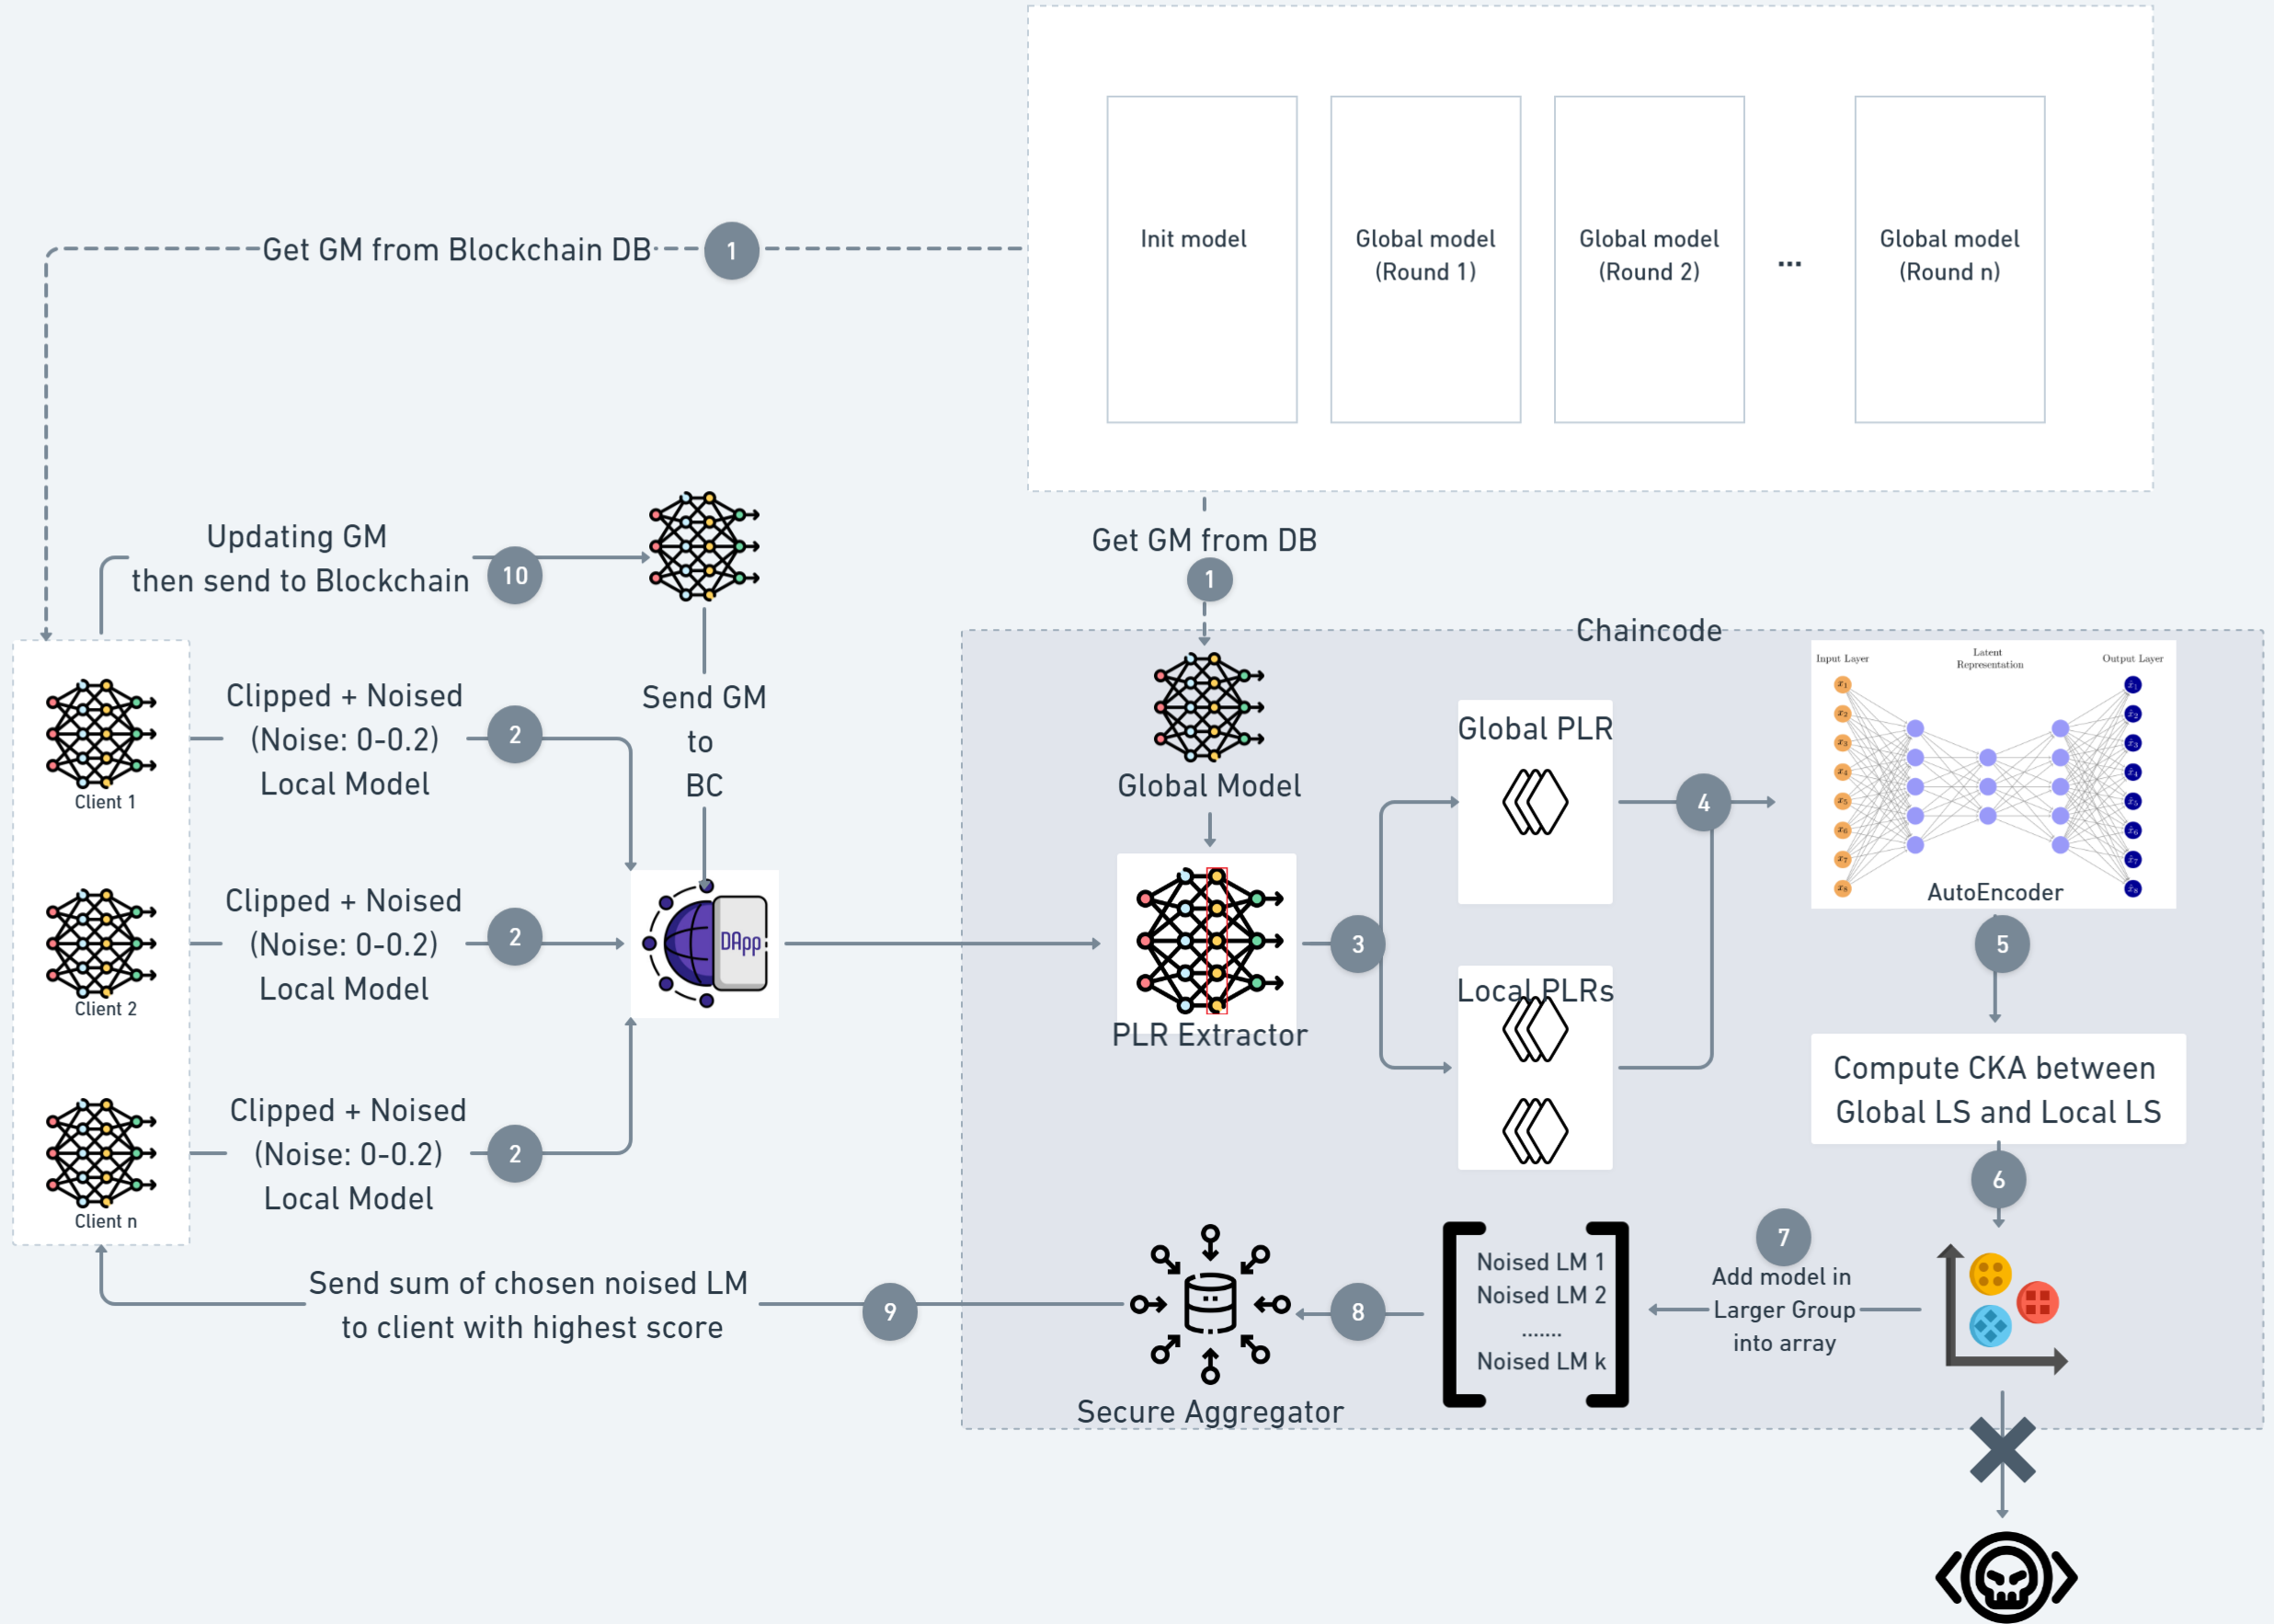
\includegraphics[width=\textwidth]{images/ArquitecturaPentidef.png}
                \caption{Arquitectura PenTiDef}
            \end{figure}
        \end{column}
    \end{columns}
\end{frame}

% --- 3. Principios de Funcionamiento (Sección 4.1.2) ---
\begin{frame}{4.1.2 Principios de Funcionamiento}{Algoritmo y Flujo de Trabajo}
    \begin{enumerate}
        \item \textbf{Recuperación:} Los clientes obtienen el modelo global (GM) de la blockchain.
        \item \textbf{Entrenamiento y Ruido:} Entrenamiento local seguido de perturbación por ruido DDP.
        \item \textbf{Extracción PLR:} Los modelos enviados extraen sus representaciones de la penúltima capa.
        \item \textbf{Reducción LSR:} El AutoEncoder comprime las PLR para mayor estabilidad ante datos no-IID.
        \item \textbf{Similitud CKA:} Se calcula la similitud entre el GM y los modelos locales.
        \item \textbf{Clustering:} KMeans divide los modelos en grupos mayoritarios (benignos) y minoritarios (atacantes).
        \item \textbf{Agregación:} Solo los modelos benignos se combinan mediante el \textit{Secure Aggregator}.
        \item \textbf{Actualización:} El cliente más confiable propaga el nuevo GM a la red.
    \end{enumerate}
\end{frame}

% --- 4. DDP con Nivel de Ruido Aleatorio (Sección 4.2) ---
\begin{frame}{4.2 DDP con Nivel de Ruido Aleatorio}{Privacidad Diferencial Distribuida}
    \begin{itemize}
        \item \textbf{Mecanismo Gaussiano:} Se define como $\mathcal{M}(w) = w + \mathcal{N}(0, \sigma^2)$ para proteger los pesos locales.
    \end{itemize}
    \begin{exampleblock}{Aleatoriedad de $\sigma$}
        Para evitar que los adversarios infieran patrones de ruido, PenTiDef selecciona $\sigma$ aleatoriamente del intervalo $[0, 0.2]$ en cada ronda.
    \end{exampleblock}
    \begin{itemize}
        \item \textbf{Beneficio:} Previene ataques de reconstrucción.
        \item \textbf{Transparencia:} Los niveles de ruido se registran en la blockchain para auditoría.
    \end{itemize}
\end{frame}

% --- 5. Integración de Blockchain (Sección 4.3) ---
\begin{frame}{4.3 Integración de Blockchain}{Coordinación en Federated Learning}
    \begin{itemize}
        \item \textbf{Hyperledger Fabric:} Red permisionada (ni pública ni anónima) de 3 organizaciones y 6 nodos pares para mayor tolerancia a fallos.
        \item \textbf{Gestión de Identidad:} Uso de certificados digitales $(ID_i, SK_i)$ para firmar transacciones y asegurar autenticidad.
        \item \textbf{Almacenamiento Híbrido:}
        \begin{itemize}
            \item \textbf{On-chain:} Hashes de los modelos $h(w_i^t)$ y metadatos de auditoría.
            \item \textbf{Off-chain:} Parámetros del modelo almacenados en \textbf{IPFS} para evitar cuellos de botella.
        \end{itemize}
        \item \textbf{Transparencia:} Garantiza que solo actualizaciones verificadas entren en el estado de aprendizaje global.
    \end{itemize}
\end{frame}